\documentclass[a4paper]{article}

\usepackage{pgfplots}
\usepgfplotslibrary{patchplots}

\begin{document}

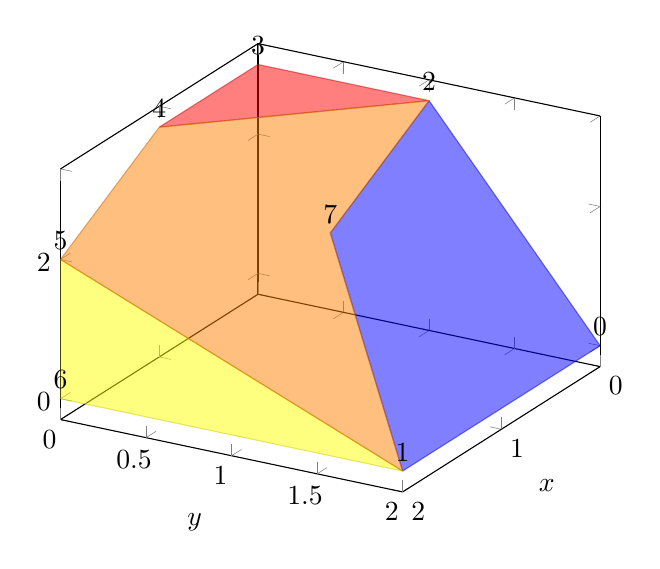
\begin{tikzpicture}
	\begin{axis}[view/h=120,xlabel=$x$,ylabel=$y$]
	\addplot3[
		opacity=0.5,
		table/row sep=\\,
		patch,
		patch type=polygon,
		vertex count=5,
		patch table with point meta={%
			0 1 7 2 2 0\\
			1 6 5 5 5 1\\
			1 5 4 2 7 2\\
			2 4 3 3 3 3\\
	}]
	table {
		x y z\\
		0 2 0\\%0
		2 2 0\\%1
		0 1 3\\%2
		0 0 3\\%3
		1 0 3\\%4
		2 0 2\\%5
		2 0 0\\%6
		1 1 2\\%7
	};
		\addplot3[only marks,nodes near coords=\coordindex]
	table[row sep=\\] {
		x y z\\
		0 2 0\\%0
		2 2 0\\%1
		0 1 3\\%2
		0 0 3\\%3
		1 0 3\\%4
		2 0 2\\%5
		2 0 0\\%6
		1 1 2\\%7
	};

	\end{axis}
\end{tikzpicture}
\end{document}

